\chapter{Rezultate}\label{Rezultate}
\section{Rezultate Experiment: comparație senzori "Fork" și "FoW"}\label{ResultsFowVsFork}
În Fig.\ref{fig:averageFoW} și Fig.\ref{fig:averageFork} putem vedea cum progresează fitness-ul mediu al populației (cu roșu) și fitness-ul celui mai bun individ din populație (cu albastru).
Aceste prime date servesc ca un proof of concept pentru faptul că algoritmul NEAT este capabil să dezvolte în populația de pradă comportamente care îi măresc fitness-ul pe parcursul evoluției (colectarea fragmentelor de energie și evitarea pereților), deoarece observăm o creștere atât a fitness-ului mediu cât și cel al celui mai bun membru din populație.
Totuși, din cele două tipuri de senzori, "FoW" se arată a fi cel mai bun, chiar dacă media este similară cu cea a populației care folosește "Fork". Fitness-ul maxim atins de creaturile cu senzor "FoW" este mai mare, ceea ce ne arată că acestea au un potențial mai mare pentru evoluție.
Pe lângă asta, putem observa în Fig.\ref{fig:connectionsFow} și Fig.\ref{fig:connectionsFork} faptul că numărul de conexiuni pentru cel mai bun membru din populația ce folosește "FoW" în ultimele generații este mai mare decât pentru populația "Fork", deci s-ar putea ca senzorul "FoW" să beneficieze mai mult de pe urma adăugării de structuri noi.

\begin{figure}[h]
	\centering
	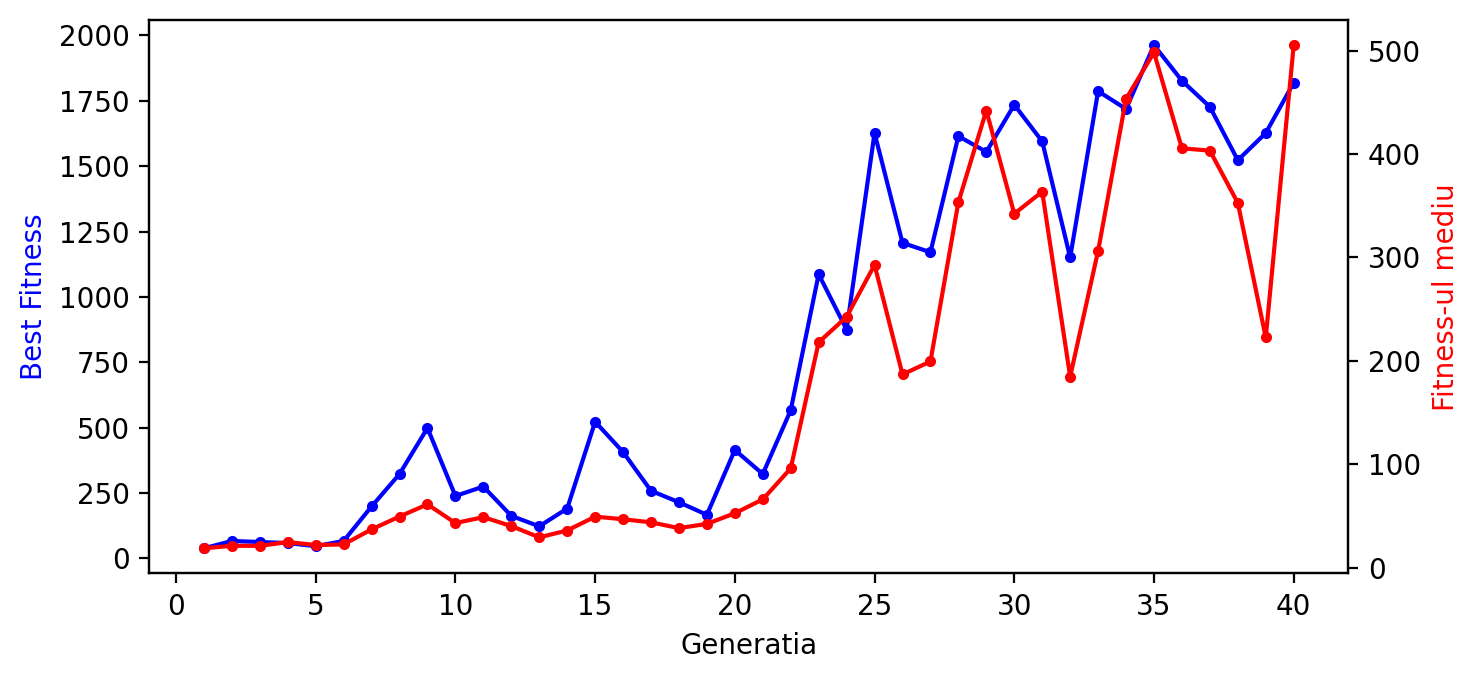
\includegraphics[width=1\textwidth]{images/experiment_fow_average.png}
	\caption{Progresia fitness-ului celui mai bun membru si a fitnessului mediu a populației pe parcursul generațiilor, pentru populații dotate cu senzorul "FoW"}
	\label{fig:averageFoW}
\end{figure}
\begin{figure}[h]
	\centering
	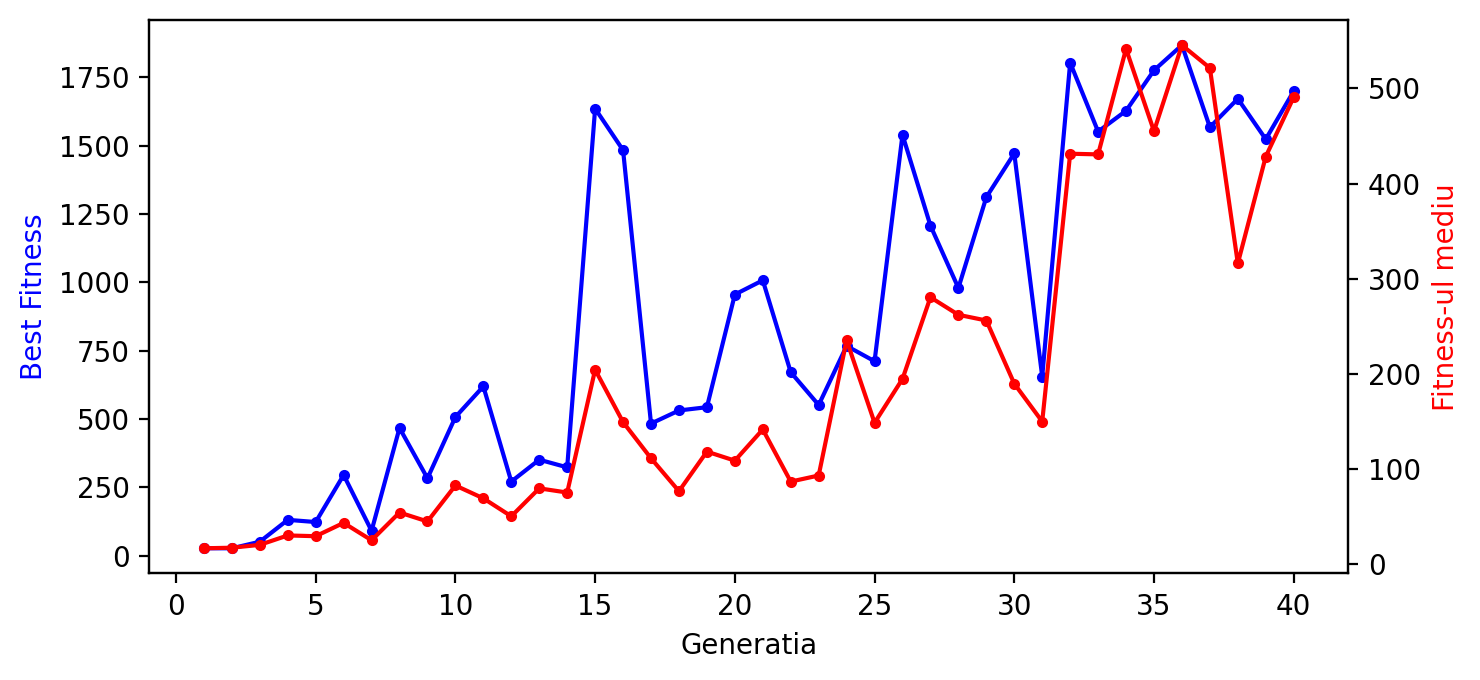
\includegraphics[width=1\textwidth]{images/experiment_fork_average.png}
	\caption{Progresia fitness-ului celui mai bun membru si a fitnessului mediu a populației pe parcursul generațiilor, pentru populații dotate cu senzorul "Fork"}
	\label{fig:averageFork}
\end{figure}
\begin{figure}[h]
	\centering
	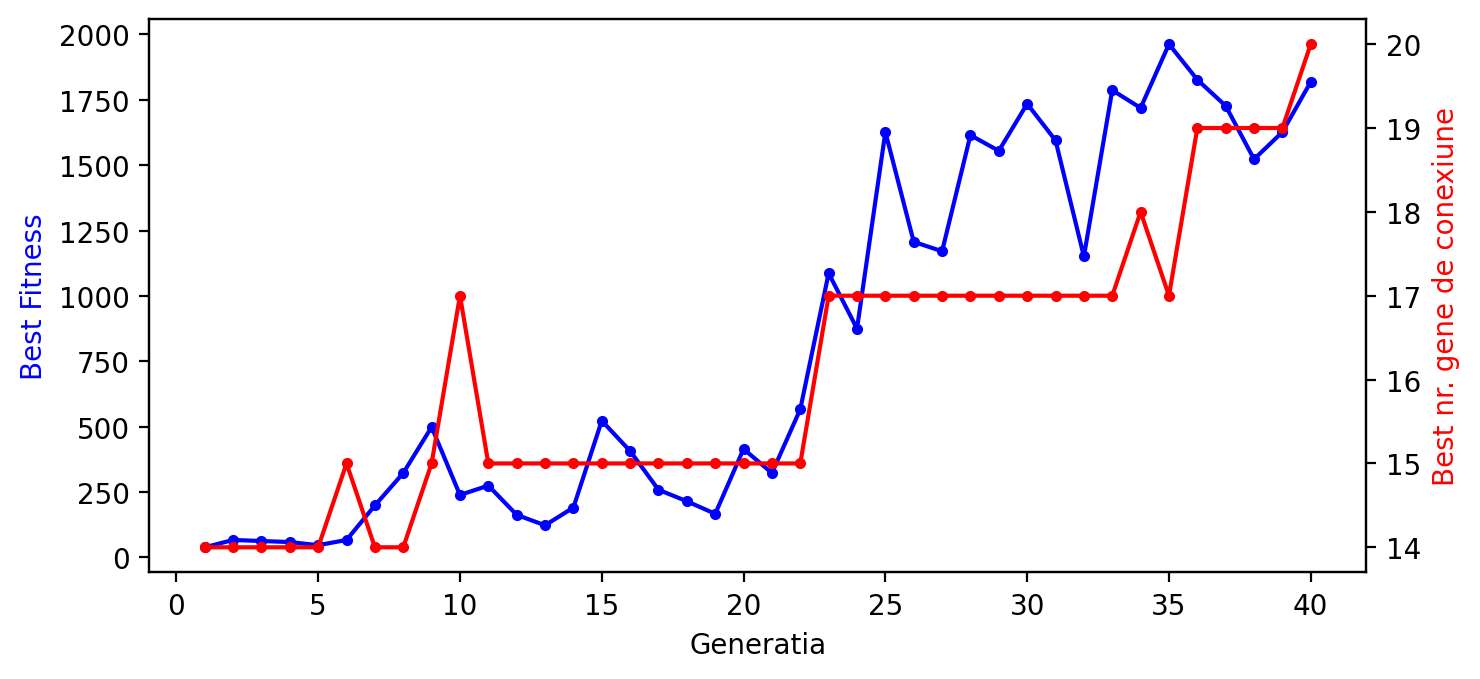
\includegraphics[width=1\textwidth]{images/experiment_fow_connections.png}
	\caption{Progresia fitness-ului celui mai bun membru si a numarului sau de gene de conexiune, pentru populații dotate cu senzorul "FoW"}
	\label{fig:connectionsFow}
\end{figure}
\begin{figure}[h]
	\centering
	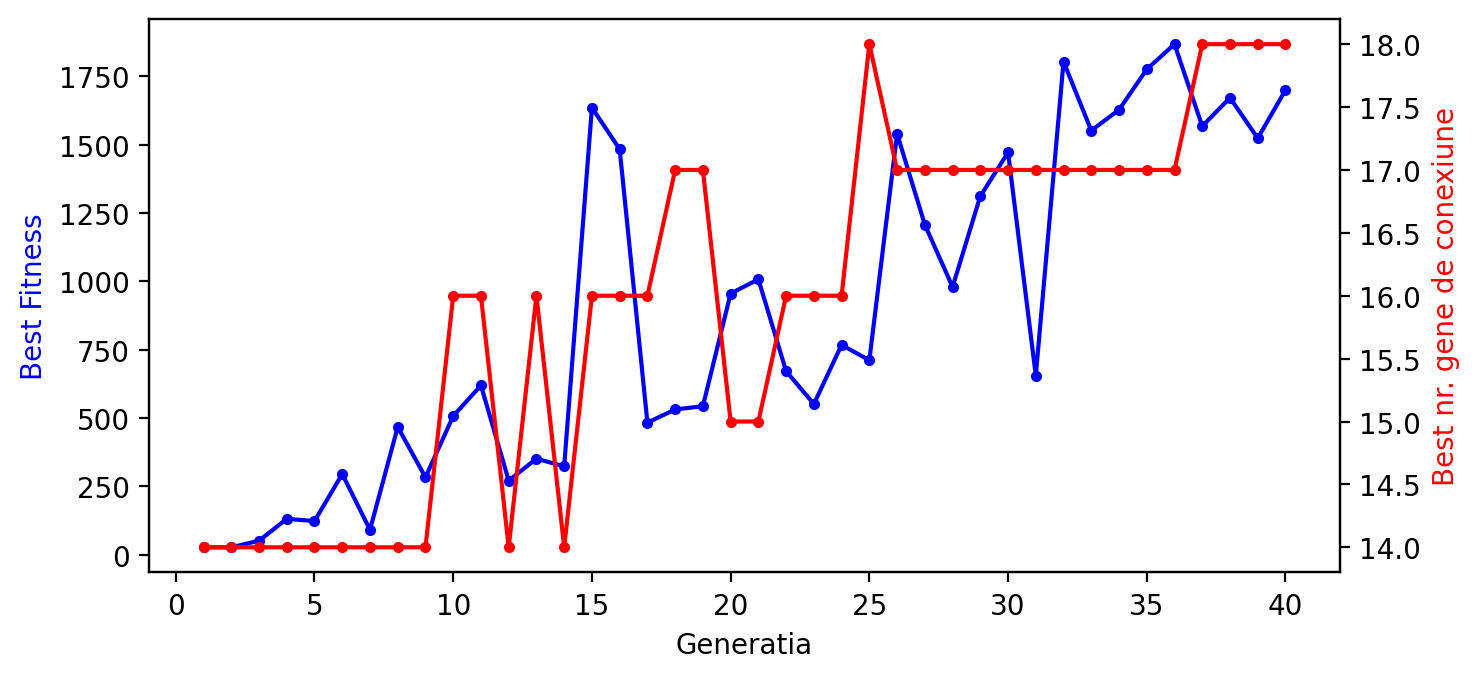
\includegraphics[width=1\textwidth]{images/experiment_fork_connections.png}
	\caption{Progresia fitness-ului celui mai bun membru si a numarului sau de gene de conexiune, pentru populații dotate cu senzorul "Fork"}
	\label{fig:connectionsFow}
\end{figure}

\section{Rezultate Experiment: comparație între păstrarea numerelor de inovație permanent sau resetarea lor la fiecare generație}\label{ResultsPermanentVsReset}
Rezultatele din această secțiune sunt pentru configurarea algoritmului în care lista numerelor de inovație este golită la începutul fiecărei generații, adică nu avem informații despre inovațiile create în generațiile anterioare.
Rezultatele pentru scenariul în care inovațiile sunt păstrate permanent le vedem în secțiunea anterioară, Fig.\ref{fig:averageFoW} și Fig.\ref{fig:connectionsFow}.
Rezultatele ne-au surprins, deoarece presupuneam că scenariul de păstrare în mod permanent al inovațiilor va duce la mai puține specii care sunt mai optimizate și consecvente.
Totuși, din Fig.\ref{fig:averageFoW} și Fig.\ref{fig:averageInov}, se vede clar că atât valorile fitness-ului mediu cât și ale celui mai bun membru sunt mai mari în scenariul curent, nu în cel precedent.
Pe lângă asta, aceste rezultate se ating și printr-un număr de conexiuni mai mic, după cum vedem în Fig.~\ref{fig:connectionsFow} și \ref{fig:connectionsInov}.
Putem presupune că rezultatele arată astfel din cauza că, chiar dacă păstrăm inovațiile timp de mai multe generații, aceeași conexiune în cadrul unei generații și în cadrul alteia s-ar putea să conecteze structuri complet diferite, deci nu ar fi potrivit să le considerăm "matching", dar asta are loc în scenariul păstrării permanente a inovațiilor.

\begin{figure}[h]
	\centering
	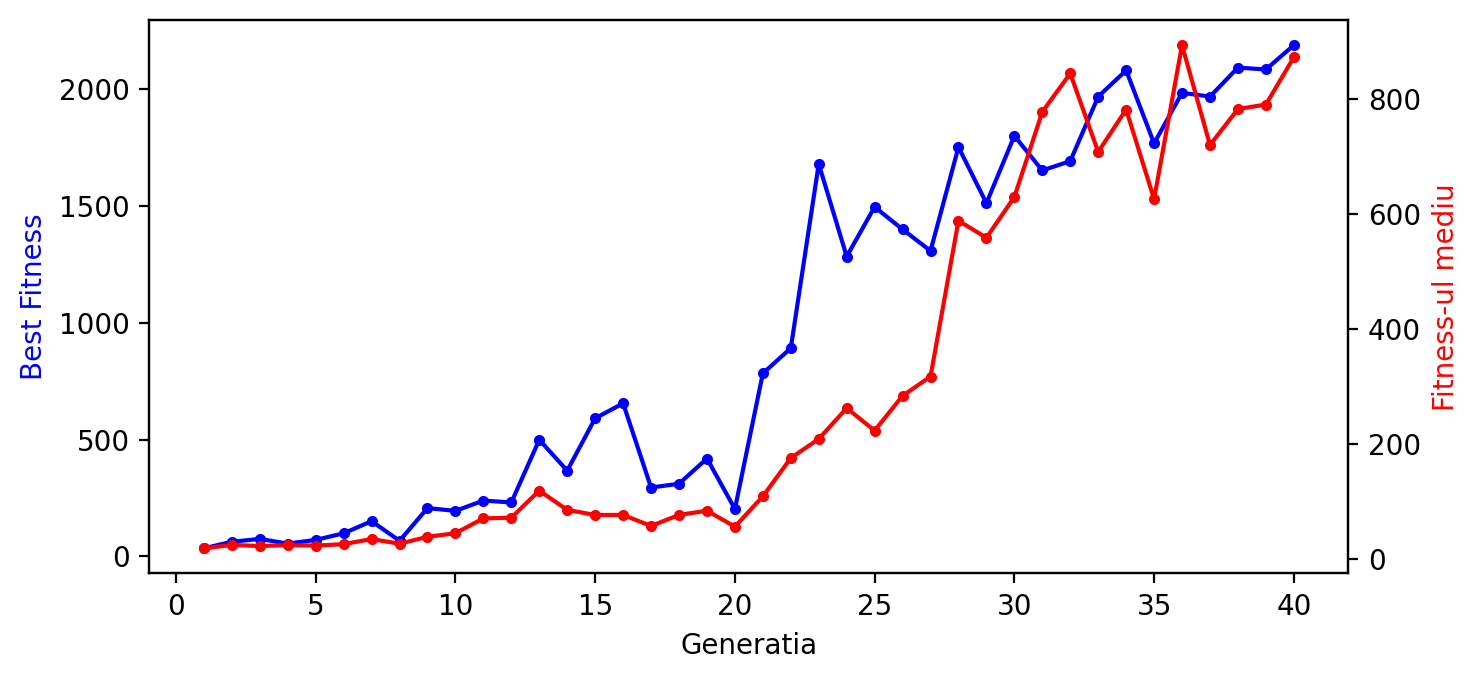
\includegraphics[width=1\textwidth]{images/experiment_inov_average.png}
	\caption{Progresia fitness-ului celui mai bun membru si a fitnessului mediu a populației pe parcursul generațiilor, in scenariul resetării numerelor de inovație}
	\label{fig:averageInov}
\end{figure}

\begin{figure}[h]
	\centering
	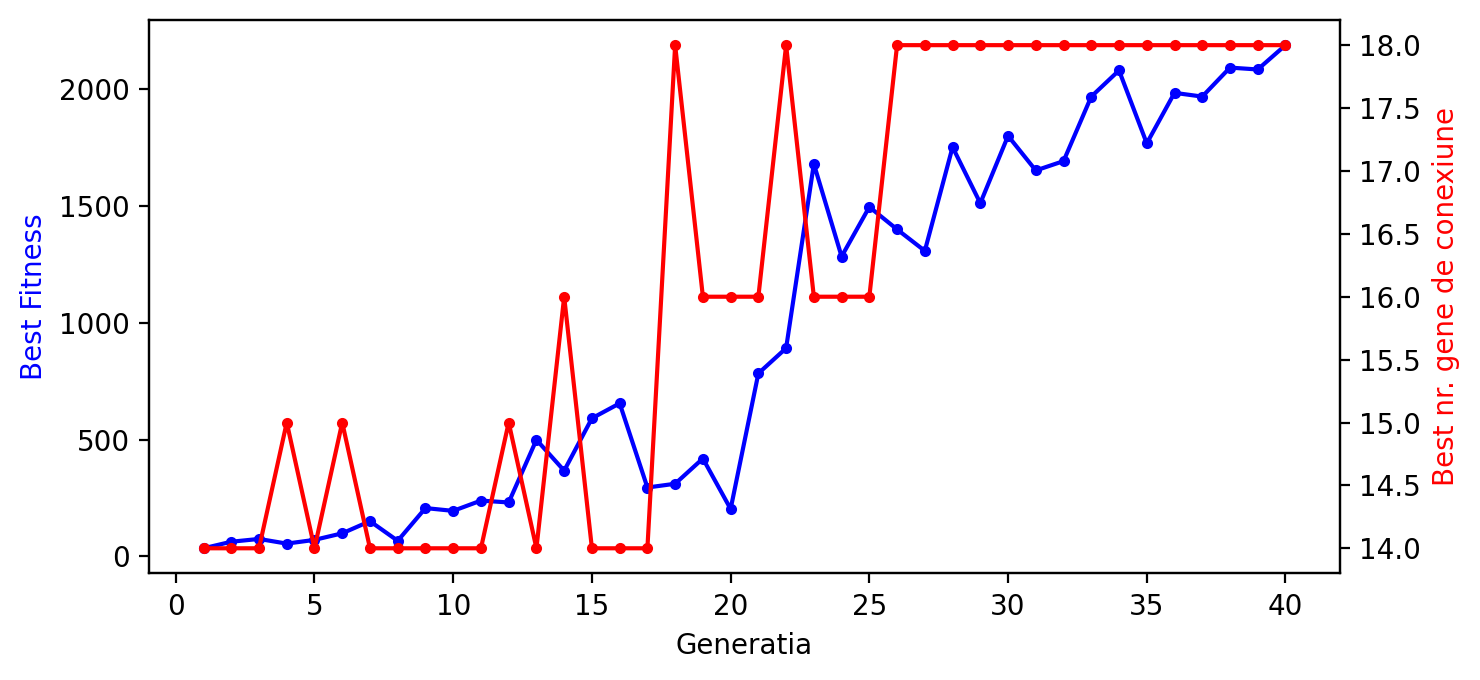
\includegraphics[width=1\textwidth]{images/experiment_inov_connections.png}
	\caption{Progresia fitness-ului celui mai bun membru si a numărului sau de gene de conexiune, in scenariul resetării numerelor de inovație}
	\label{fig:connectionsInov}
\end{figure}


\section{Rezultate Experiment: dezvoltarea comportamentelor de urmărire in prădători}\label{ResultsChassing}
Prin acest experiment am demonstrat ca utilizând NEAT, prădătorii pot să învețe comportamente de urmărire, văzând cu progresia generațiilor si o îmbunătățire a fitness-ului mediu si al celui mai bun membru, in Fig.\ref{fig:averageChassing}.\\
In Fig.\ref{fig:connectionsChassing} putem vedea si faptul ca in același timp se complica si topologia retelei
\begin{figure}[h]
	\centering
	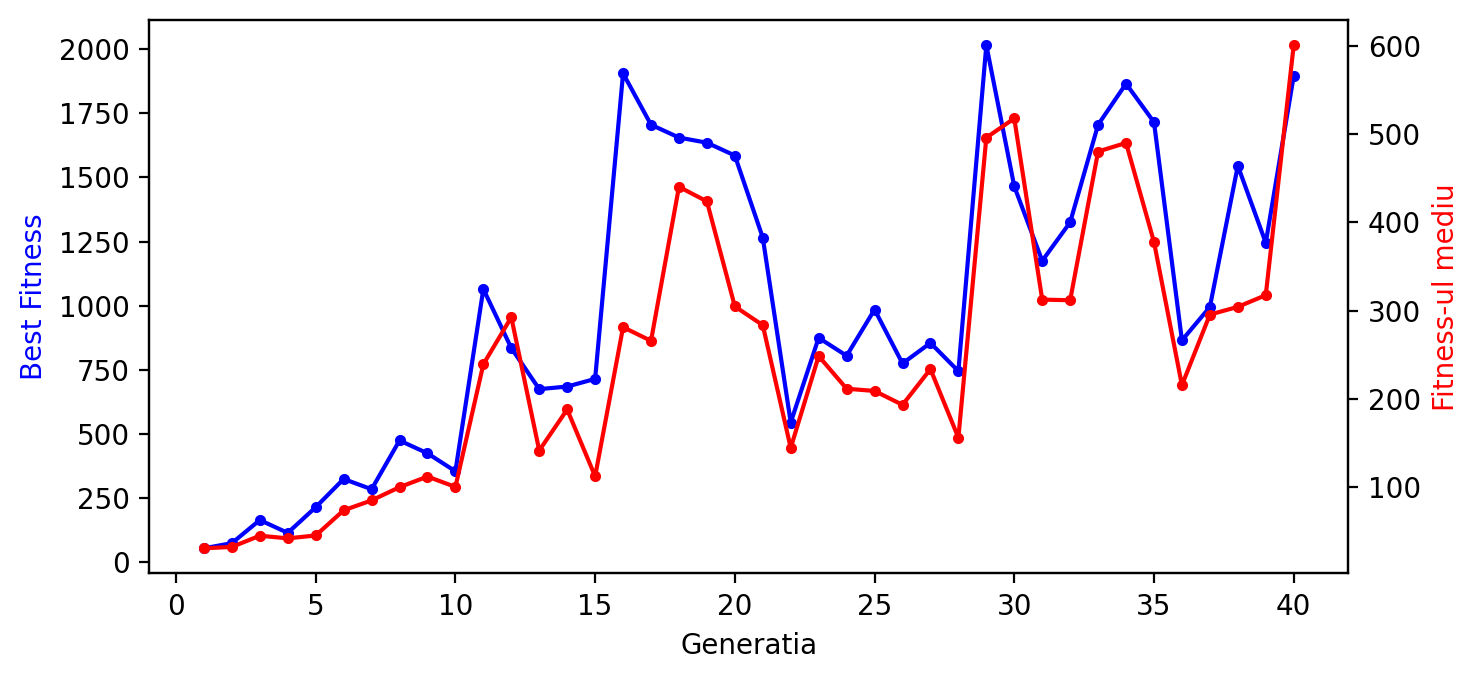
\includegraphics[width=1\textwidth]{images/experiment_chassing_average.png}
	\caption{Progresia fitness-ului celui mai bun prădător si a fitnessului mediu a prădătorilor, in scenariul de dezvoltare al comportamentelor de urmărire}
	\label{fig:averageChassing}
\end{figure}

\begin{figure}[h]
	\centering
	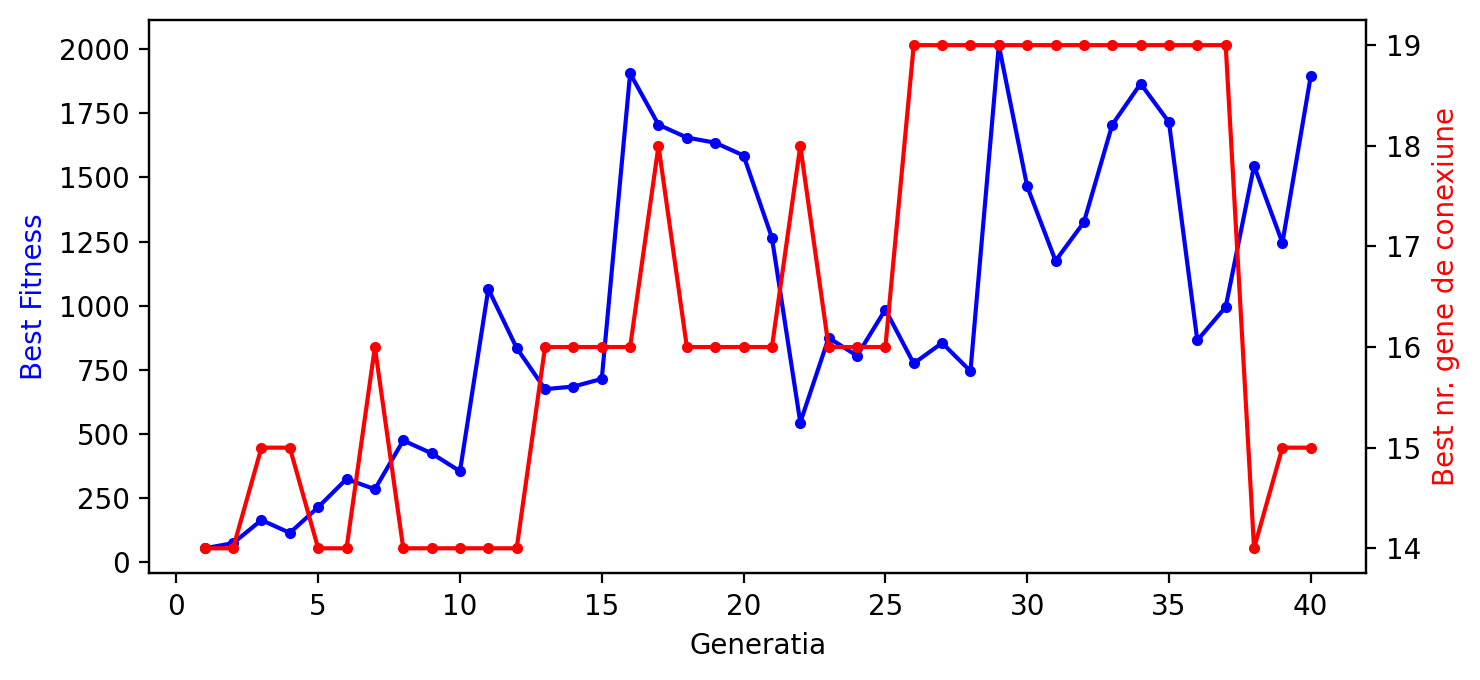
\includegraphics[width=1\textwidth]{images/experiment_chassing_connections.png}
	\caption{Progresia fitness-ului celui mai bun prădător si a numărului sau de gene de conexiune, in scenariul de dezvoltare al comportamentelor de urmărire}
	\label{fig:connectionsChassing}
\end{figure}

\section{Rezultate Experiment: coevoluția prăzii și a prădătorilor}\label{ResultsCoevolution}
Pentru acest experiment, rezultatele sunt dezamăgitoare. Cu parametrii de mediu curent nu am putut stabili o creștere perceptibilă nici pentru fitness-ul prăzii (Fig.\ref{fig:coevPreyAverage}) și nici pentru cel al prădătorilor (Fig.\ref{fig:coevPredatorAverage}).
Se pot vedea spike-uri pe alocuri, ceea ce înseamnă că sunt indivizi care au dezvoltat comportamentele potrivite, dar acestea nu sunt optimizate mai departe în populație.
Putem să vedem asta și prin faptul că apar constant mutații noi, dacă ne uităm la numărul de conexiuni ale celor mai buni membri din ambele populații (Fig.\ref{fig:coevPreyConnections} și Fig.\ref{fig:coevPredatorConnections}).

\begin{figure}[h]
	\centering
	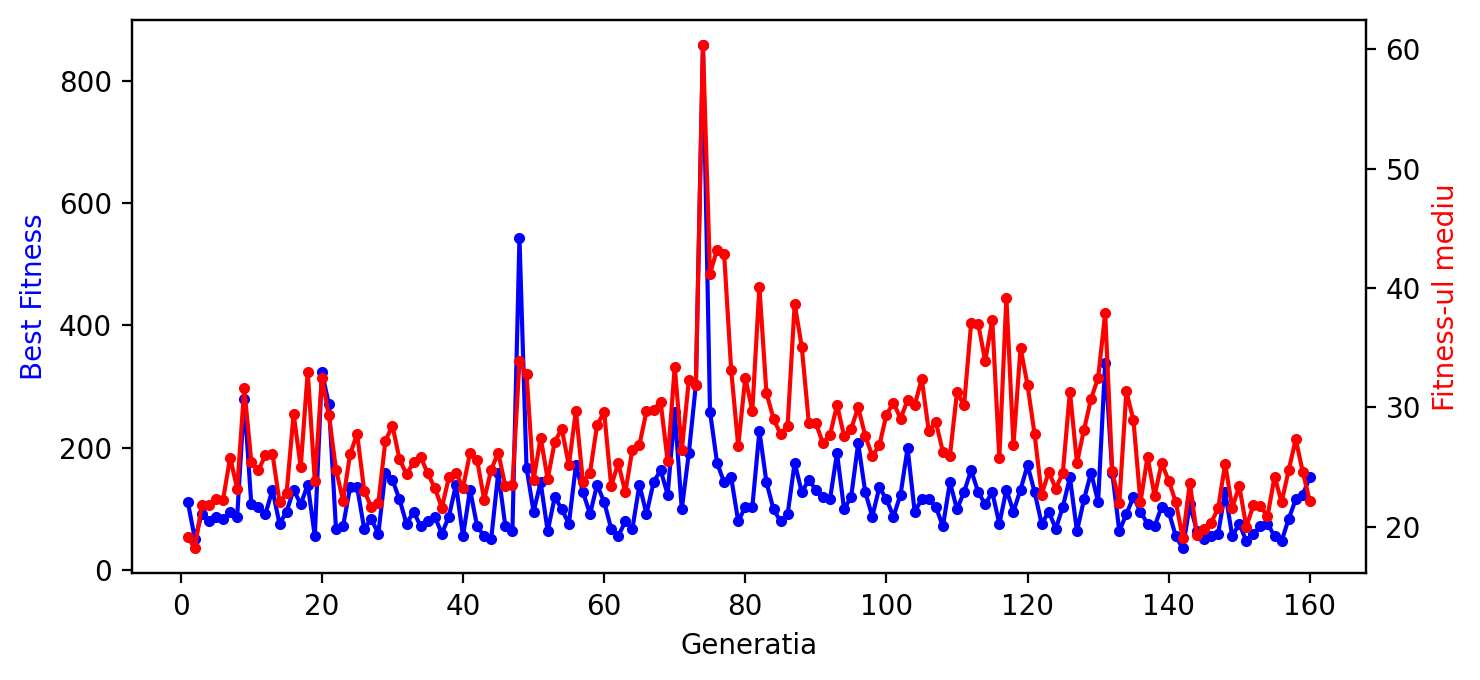
\includegraphics[width=1\textwidth]{images/coevolution_average_prey.png}
	\caption{Progresia fitness-ului celei mai bune prazi si a fitnessului mediu a prăzilor, in experimentul de coevoluție}
	\label{fig:coevPreyAverage}
\end{figure}

\begin{figure}[h]
	\centering
	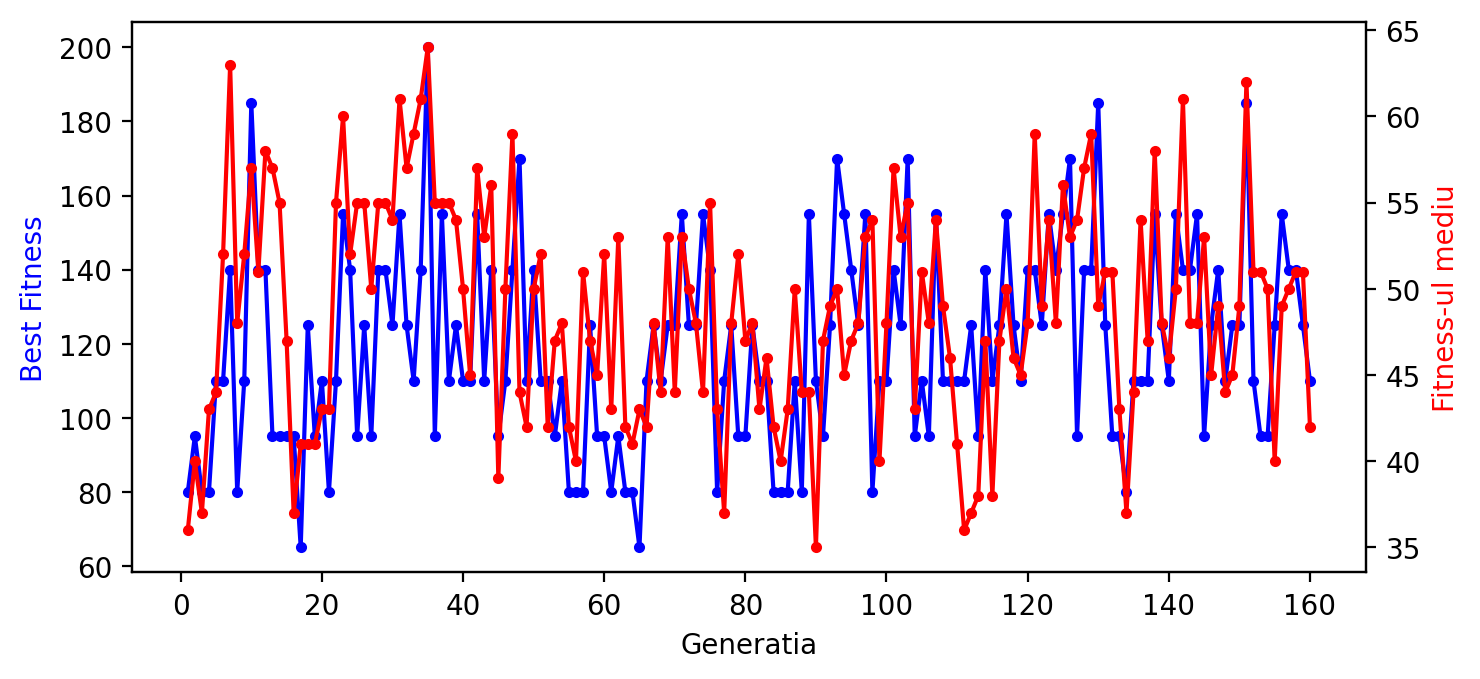
\includegraphics[width=1\textwidth]{images/coevolution_pradator_average.png}
	\caption{Progresia fitness-ului celui mai bun prădător si a fitness-ului mediu al prădătorilor, in experimentul de coevoluție}
	\label{fig:coevPredatorAverage}
\end{figure}

\begin{figure}[h]
	\centering
	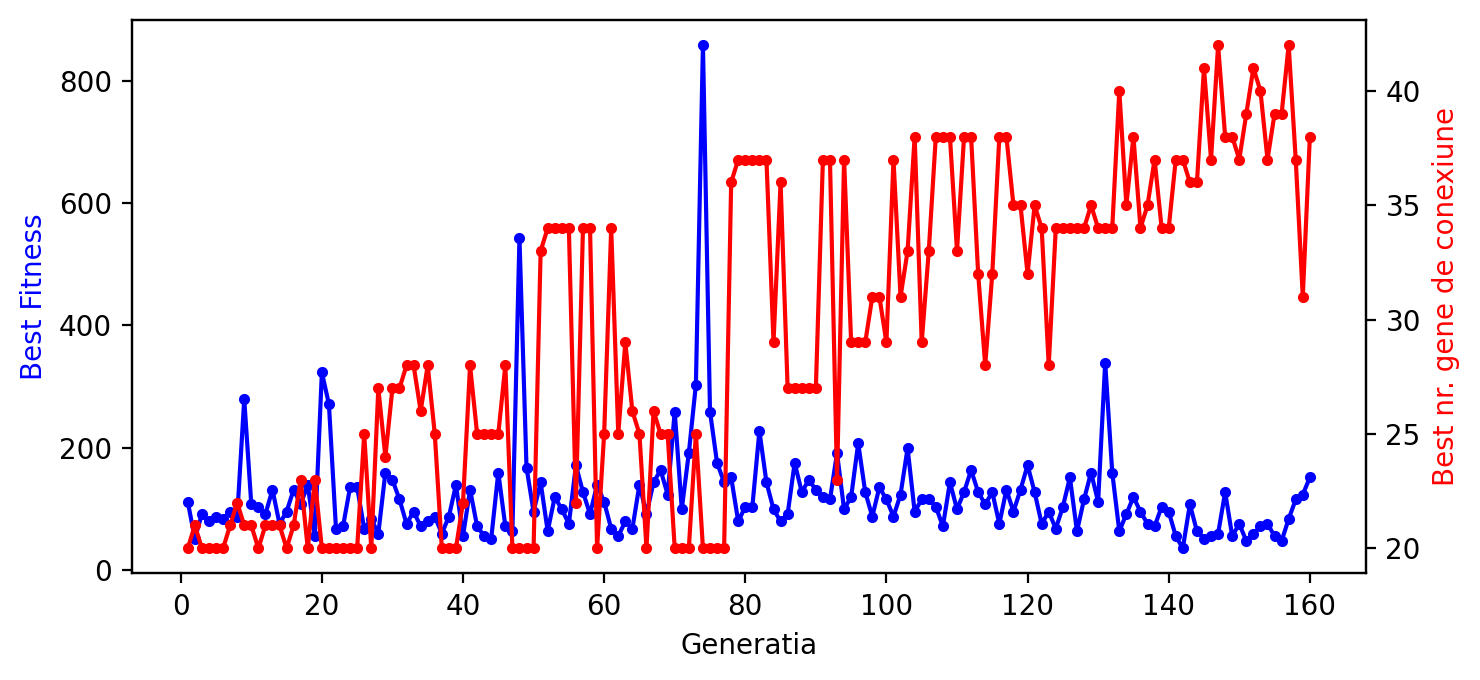
\includegraphics[width=1\textwidth]{images/coevolution_connections_prey.png}
	\caption{Progresia fitness-ului celei mai bune prazi si a numărului ei de gene de conexiune, in experimentul de coevoluție}
	\label{fig:coevPreyConnections}
\end{figure}

\begin{figure}[h]
	\centering
	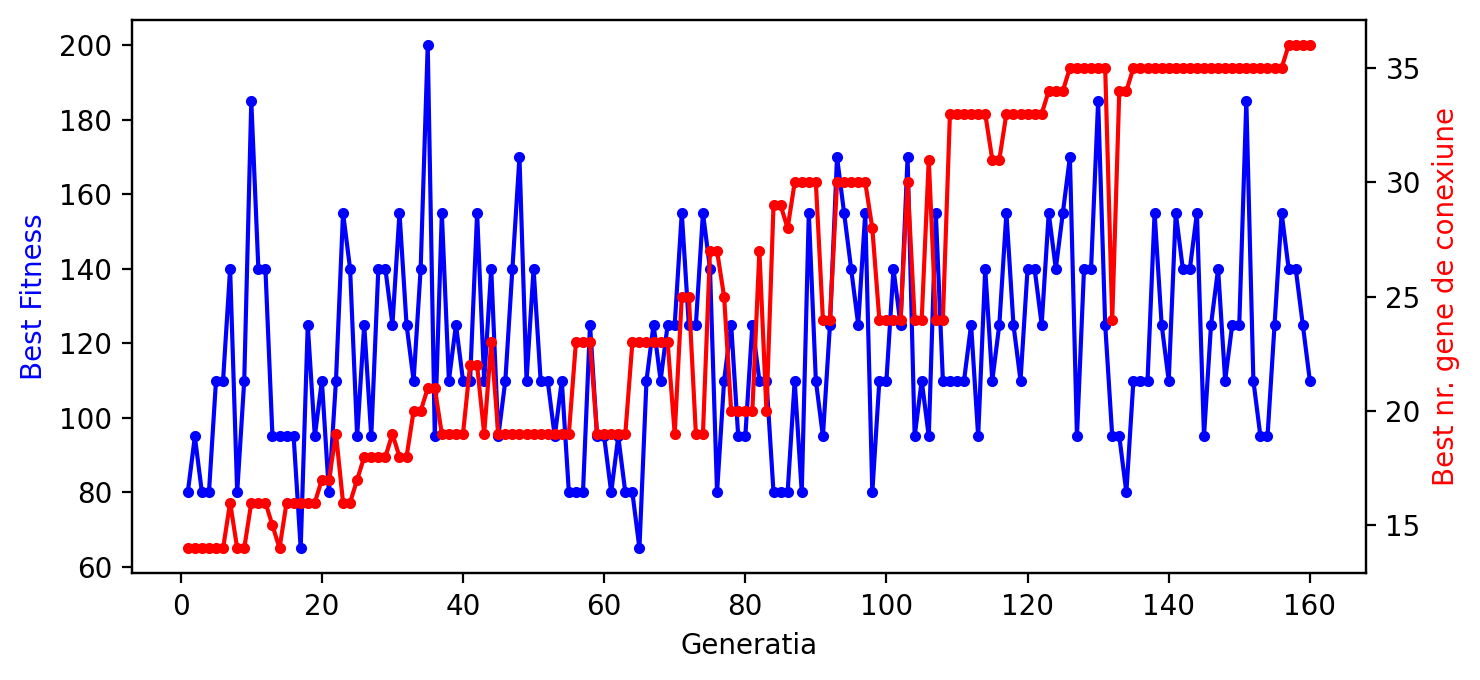
\includegraphics[width=1\textwidth]{images/coevolution_pradator_connections.png}
	\caption{Progresia fitness-ului celui mai bun prădător si a numărului sau de gene de conexiune, in experimentul de coevoluție}
	\label{fig:coevPredatorConnections}
\end{figure}